\section{Specifications}
\label{sec:specs}
\newcounter{SpecID}

\subsection{Markers}
\refstepcounter{SpecID}
\label{spec:markers}

The arena and tokens in the game are labelled with \emph{libkoki} fiducial
markers. Each marker number is associated with a particular feature in the
arena, and also has an associated size. The marker numbers and sizes are as
follows:

\begin{center}
\begin{tabular}{lcc}
  \toprule
  \textbf{Item} & \textbf{Marker Number} & \textbf{Marker Size (\si{mm})} \\
  \midrule
  Arena boundary & 0 -- 27 & 250 \\
  Tokens (gold) & 28 -- 38 & 150 \\
  Tokens (silver) & 39 -- 49 & 150 \\
  \bottomrule
\end{tabular}
\end{center}

All markers are oriented vertically such that the principal corner of the marker
(which is indicated by a dark grey dot in the black marker border) is on the
higher edge.

\subsection{Arena}
\refstepcounter{SpecID}
\label{spec:arena}

\begin{enumerate}
  \item The arena floor is an \SI{8}{m} $\times$ \SI{8}{m} square. The tolerance
        of these two dimensions is $\pm$ \SI{250}{mm}.
  \item The floor of the arena is carpeted.
  \item The layout of the arena is given in Figure~\ref{fig:arena}.
  \item The outer walls of the arena are at least \SI{600}{mm} high, and the
        interior surface is white plastic-coated hardboard.
  \item Each wall of the arena features seven \SI{250}{mm} libkoki markers.
        The positions of these markers is given in Figure~\ref{fig:sidewall}.
        The marker numbering is given in Figure~\ref{fig:arena}.
  \item TODO: robot zones
\end{enumerate}

\begin{sidewaysfigure}
  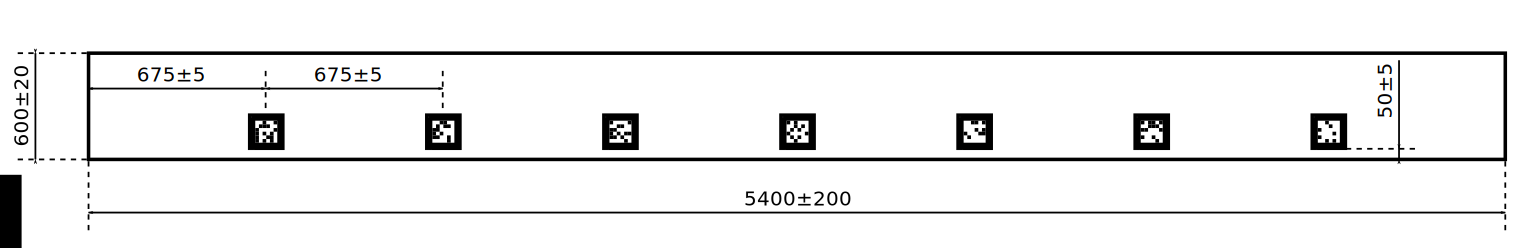
\includegraphics[scale=0.58]{fig-sidewall.pdf}
  \caption{Layout of markers along each arena wall.}
  \label{fig:sidewall}
\end{sidewaysfigure}

\begin{figure}
  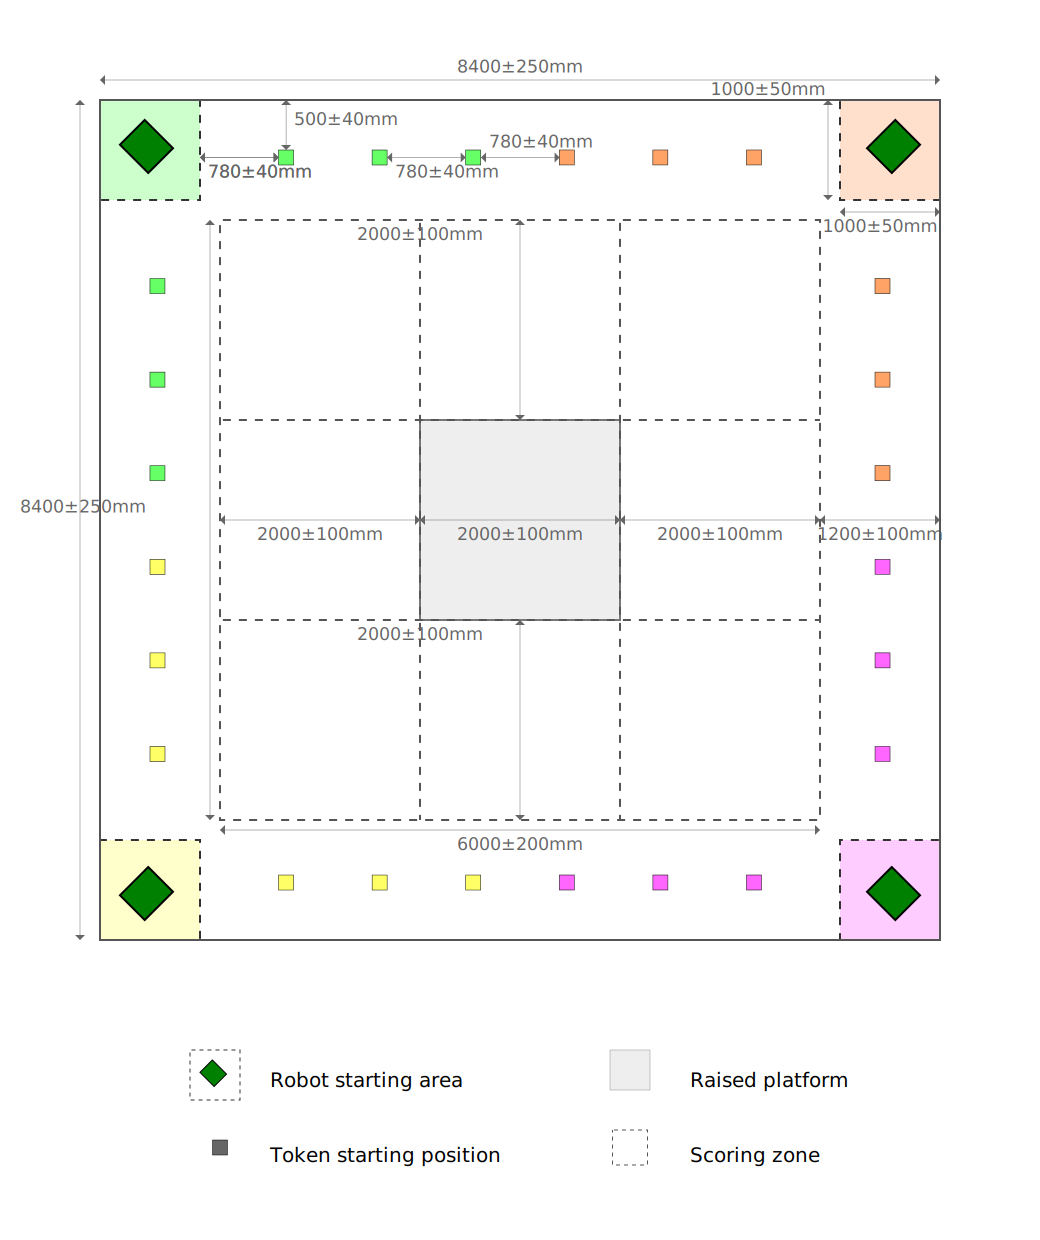
\includegraphics[scale=0.58]{fig-arena.pdf}
  \caption{Layout zones and tokens in the arena.}
  \label{fig:arena}
\end{figure}

%\subsection{Badges}
%\refstepcounter{SpecID}
%\label{spec:badges}

\subsection{Tokens}
\refstepcounter{SpecID}
\label{spec:tokens}

TODO: decide

